%%%%%%%%%%%%%%%%%%%%%%%%%%%%%%%%%%%%%%%%%%%%%%%%%%%%%%%%%%%%%%%%%%%%%%%%%%%%%%%%%%%%%%%%%%%%%%%%%%%%%%%%%%%%%%%%%%%%%%%%%%%%%%%%%%%%%%%%%%%%%%%%%%%%%%%%%%%%%%%%%%%
% Written By Michael Brodskiy
% Class: Fundamentals of Networks
% Professor: E. Bernal Mor
%%%%%%%%%%%%%%%%%%%%%%%%%%%%%%%%%%%%%%%%%%%%%%%%%%%%%%%%%%%%%%%%%%%%%%%%%%%%%%%%%%%%%%%%%%%%%%%%%%%%%%%%%%%%%%%%%%%%%%%%%%%%%%%%%%%%%%%%%%%%%%%%%%%%%%%%%%%%%%%%%%%

\documentclass[12pt]{article} 
\usepackage{alphalph}
\usepackage[utf8]{inputenc}
\usepackage[russian,english]{babel}
\usepackage{titling}
\usepackage{amsmath}
\usepackage{graphicx}
\usepackage{enumitem}
\usepackage{amssymb}
\usepackage[super]{nth}
\usepackage{everysel}
\usepackage{ragged2e}
\usepackage{geometry}
\usepackage{multicol}
\usepackage{fancyhdr}
\usepackage{cancel}
\usepackage{siunitx}
\usepackage{physics}
\usepackage{tikz}
\usepackage{mathdots}
\usepackage{yhmath}
\usepackage{cancel}
\usepackage{color}
\usepackage{array}
\usepackage{multirow}
\usepackage{gensymb}
\usepackage{tabularx}
\usepackage{extarrows}
\usepackage{booktabs}
\usepackage{lastpage}
\usepackage{float}
\usetikzlibrary{fadings}
\usetikzlibrary{patterns}
\usetikzlibrary{shadows.blur}
\usetikzlibrary{shapes}

\geometry{top=1.0in,bottom=1.0in,left=1.0in,right=1.0in}
\newcommand{\subtitle}[1]{%
  \posttitle{%
    \par\end{center}
    \begin{center}\large#1\end{center}
    \vskip0.5em}%

}
\usepackage{hyperref}
\hypersetup{
colorlinks=true,
linkcolor=blue,
filecolor=magenta,      
urlcolor=blue,
citecolor=blue,
}


\title{Conceptual Homework 4}
\date{December 4, 2023}
\author{Michael Brodskiy\\ \small Professor: E. Bernal Mor}

\begin{document}

\maketitle

\begin{enumerate}

    \item List 2 services that the link layer can offer to the network layer and have corresponding services in TCP.

      One example of such a service is flow control. With the link layer, nodes have limited capacity to act as a buffer, thus requiring a method to prevent buffer overflow (and, consequently, frame loss). To prevent this, a link layer service may be implemented to control the rate at which the sending node releases frames so as not to overwhelm the receiving node. Congruently, TCP implements flow control as well (in different ways, depending on the flavor of TCP). Another example of such a service would be reliable delivery. When the link layer implements reliable delivery, it guarantees that a frame will arrive at the receiver. The method in which reliable delivery is implemented in the link layer is similar to the way in which it is implemented in TCP (through acknowledgements and retransmissions).

    \item Consider a broadcast channel of rate $R$ where CSMA/CD is implemented. Suppose Node A and Node B start to transmit at the same time a frame of length $L$ over the broadcast channel. Denote the propagation delay between the two nodes as $d_{prop}$.

      \begin{enumerate}

        \item Will A detect the collision if $d_{prop}>L/R$? Why or why not? Briefly explain your answer.

          In the given scenario, we know that the transmission delay will be $L/R$. We know, by definition, that the propagation delay is the time for a bit to travel from source to destination. Thus, we can say that a collision will occur when $d_{prop}>L/R$, which means that, in the given situation we know there is a collision.\\

          Next, we must define the requirements for collision detection. For CSMA/CD to detect a collision, we know that the following condition must be satisfied:

          $$d_{trans}\geq 2d_{prop}$$
          $$\frac{L}{R}\geq 2d_{prop}$$

          Since, with our values, this is never true, the collision is not detected

        \item If you were to design a CSMA/CD protocol for this broadcast channel, what would you do to make sure that all the collisions are detected in the transmitters?

          As evident from the problem above, the collision has trouble being detected because of the large propagation delay. This, in tandem with the fact that CSMA/CD is used in wired networks only, can be key in fixing the issue. We know the propagation delay to be:

          $$d_{prop}=\frac{d}{s}$$

          Thus, we may fix the issue by either decreasing the wired link length, or obtaining a cable in which the propagation speed is greater. As such, the CSMA/CD protocol would be able to more easily detect a collision within the channel.

       \end{enumerate}

    \item In Ethernet CSMA/CD with exponential backoff, after the fifth collision, what is the probability that a node chooses $K = 4$? The result $K = 4$ corresponds to a delay of how many seconds on a $100$Mbps Ethernet?

      Since it is given that a fifth collision has occurred, we may write:

      $$\boxed{2^5=32\to p=\frac{1}{32-1}=.032258}$$

      The delay may be expressed as the product of $K$, 512, and the transmission time for a bit:

      $$d=(5)(512)\left( \frac{1}{100\cdot10^6} \right)$$
      $$\boxed{d=20.48[\si{\micro\second}]}$$

    \item Plot the following figures:

      \begin{enumerate}

          \item A figure that shows the efficiency (probability any node has a success) as a function of the transmission probability $p$ for slotted ALOHA. Include three curves that correspond with the following values of the number of nodes, $N: N=15,N=25, N=35$.

            \begin{figure}[H]
              \centering
              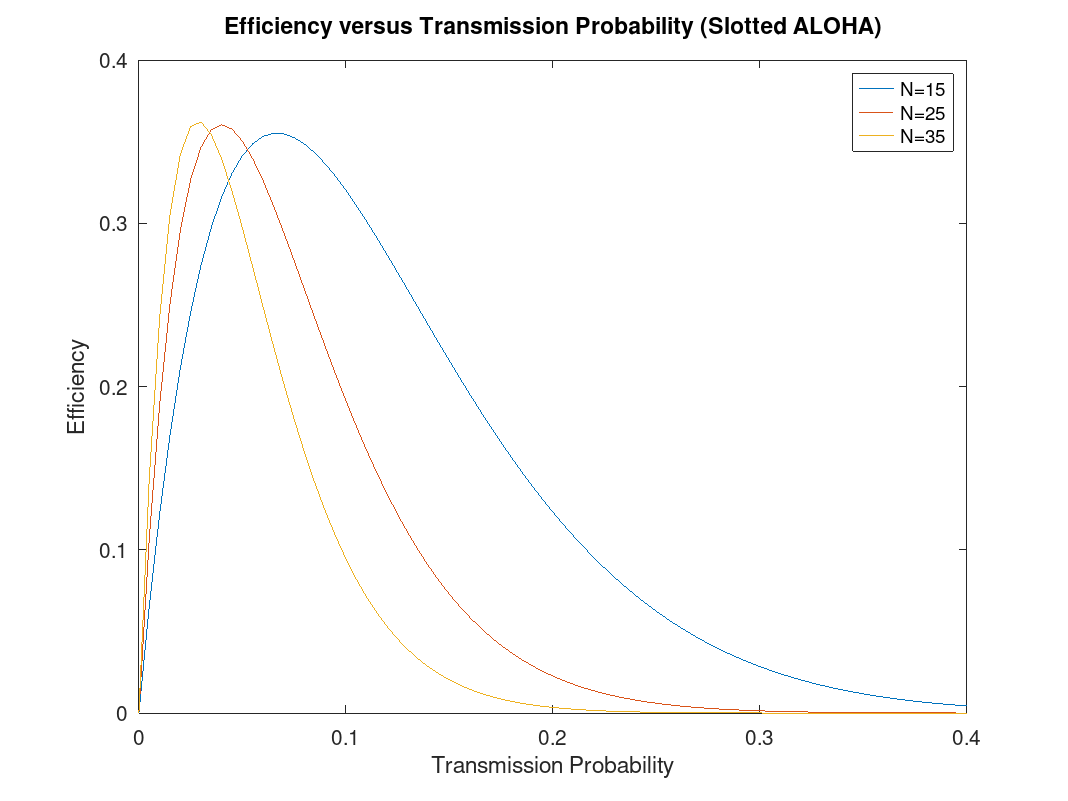
\includegraphics[width=.7\textwidth]{Figures/SlottedAloha.png}
              \caption{Slotted Aloha Plot for $N=15,25,35$}
              \label{fig:1}
            \end{figure}

            Note that, as expected, the efficiency is maximized at approximately $\dfrac{1}{e}\approx.37$

          \item Same figure for pure ALOHA.

            \begin{figure}[H]
              \centering
              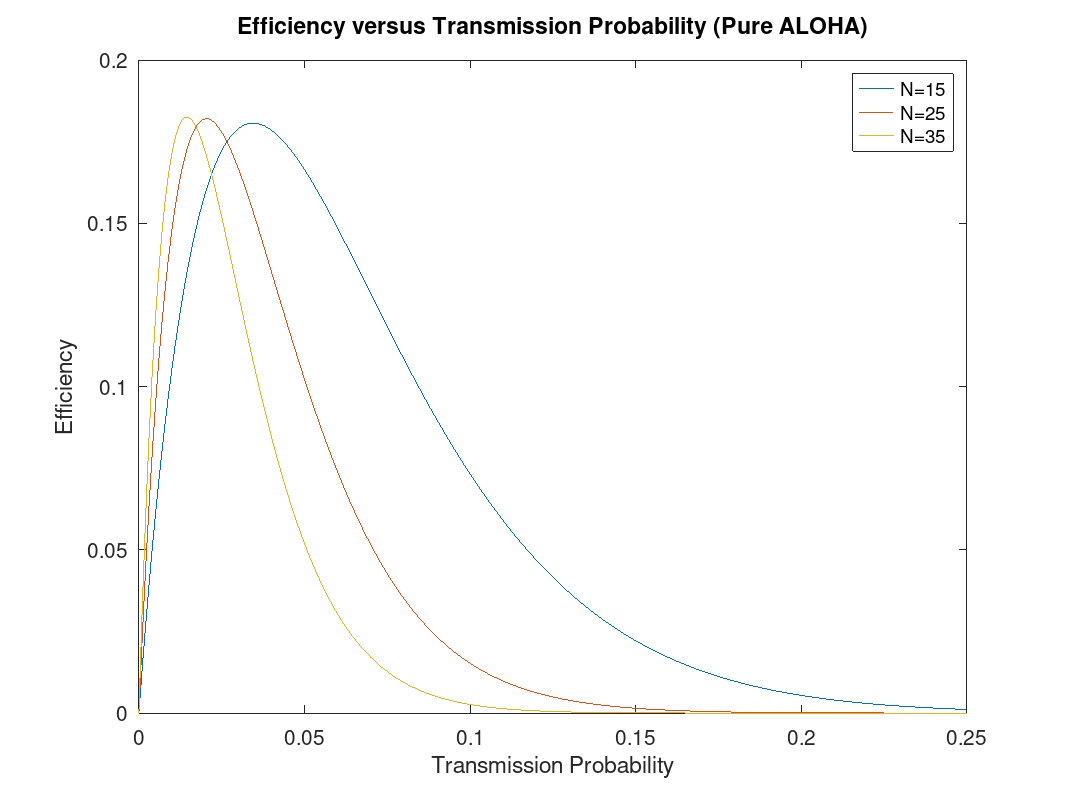
\includegraphics[width=.7\textwidth]{Figures/PureAloha.png}
              \caption{Pure Aloha Plot for $N=15,25,35$}
              \label{fig:2}
            \end{figure}

            Note that, as expected, the efficiency is maximized at approximately $\dfrac{1}{2e}\approx.18$

      \end{enumerate}

    \item Why is an ARP query sent within a broadcast frame? Why is an ARP response sent within a frame with a specific destination MAC address?

      ARP is used for local area network (LAN) discovery. Given a node that wants to find another node within a LAN, the only information the searching node has is the IP address. Thus, the searching node launches an ARP broadcast for another node with a corresponding IP address. The node being searched for then receives this broadcast query frame. The query frame contains both the IP and MAC addresses of the searching node. Thus, the node being searched for responds, this time directly to the MAC address of the searching node, with its MAC address.

\end{enumerate}

\end{document}

